\documentclass[a4paper,12pt]{report}
\usepackage{color}
\usepackage{hyperref}
\hypersetup{
    colorlinks,
    citecolor=black,
    filecolor=black,
    linkcolor=black,
    urlcolor=black
}
\setcounter{secnumdepth}{0}
\usepackage{graphicx}
\usepackage{epstopdf}
\usepackage{amsmath}
\usepackage[table,xcdraw]{xcolor}
\usepackage{amssymb}
\usepackage{listings}
\definecolor{anti-flashwhite}{rgb}{0.95, 0.95, 0.96}
\lstset{ 
  backgroundcolor=\color{anti-flashwhite}
  }
\begin{document}
\title{
\textbf{Operating Systems - II: CS3523}\\~\\
\begin{large}
\textbf{Programming Assignment - III\\~\\Solving Producer Consumer Problem\\using Semaphores
\& Locks\\}
\end{large}
\begin{large}
\textbf{Assignment Report}
\end{large}
}
\author{\textbf{Sagar Jain - CS17BTECH11034}\\}
\maketitle
\begin{large}
\tableofcontents
\end{large}
\newpage
\section{Salient Features of Program Design}
The problem has been solved using semaphores and locks.
\subsection{Semaphores}
Semaphores have been implemented using the header \textbf{\textit{semaphore.h}}
\begin{enumerate}
\item I have used three semaphores, \textbf{\textit{full}}, \textbf{\textit{empty}} and \textbf{\textit{locker}}.
\item \textbf{\textit{locker}} is initialised as 1, \textbf{\textit{full}} as 0 and \textbf{\textit{empty}} as the capacity of the buffer.
\item \textbf{\textit{full}} is used in the consumer thread to ensure that no consumer can consume if there are no full buffers and we increment it in the producer thread everytime something is produced.
\item \textbf{\textit{empty}} is used in the producer thread to ensure that no producer can produce if there are no empty buffers and we decrement it in the consumer thread everytime something is consumed.
\item \textbf{\textit{locker}} is used to ensure mutual exclusion between multiple producers and consumers.
\end{enumerate}
\subsection{Locks}
Mutex has been implemented using the header \textit{\textbf{mutex}}.
\begin{enumerate}
\item I have used two locks \textbf{\textit{check\_lock}} and \textbf{\textit{update\_lock}}. \textbf{\textit{counter}} is used to keep the count of the number of filled buffer cells.
\item \textbf{\textit{check\_lock}} is used to ensure that no two processes read the same value of counter and update them leading to a race condition.
\item \textbf{\textit{update\_lock}} is used to ensure that no two processes are reading and weiting at the same time.
\item \textbf{\textit{check\_lock}} is unlocked after \textbf{\textit{update\_lock}} to make sure that another thread can only check the condition once current thread has updated the value of \textit{\textbf{counter}}.
\end{enumerate}
\newpage
\section{Program Output}
The programs output log files (\textit{output-semaphore.txt}, \textit{output-lock.txt}). These files have the data about the point in time at which any consumer or producr consumes or produces any item from or into the buffer.
For Example:\\\\
\textit{14th item produced by thread 4 at 19:58:09 into buffer location 61\\
0th item read from the buffer by thread 0 at 19:58:09 from buffer location 60\\
1th item read from the buffer by thread 0 at 19:58:11 from buffer location 59}
\newpage
\section{Results \& Graphs}

\begin{center}
\begin{large}
\textbf{Average Waiting Time vs Number of Threads}
\end{large}
%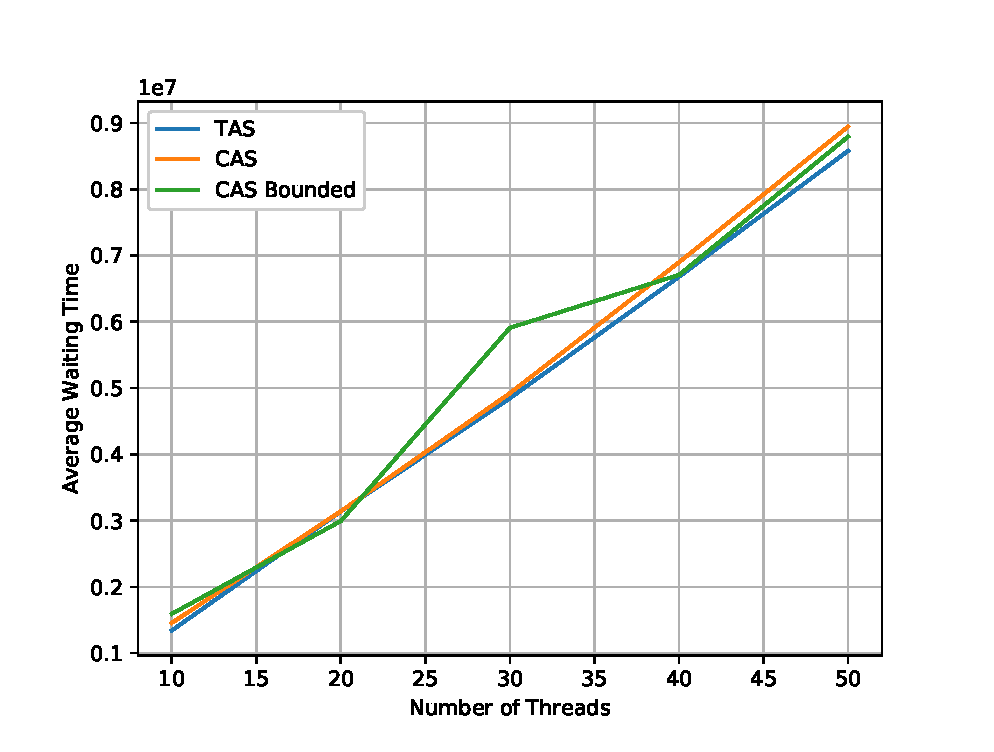
\includegraphics{avg.eps}
\end{center}
\begin{center}
\begin{large}
\textbf{Maximum Waiting Time vs Number of Threads}
\end{large}
%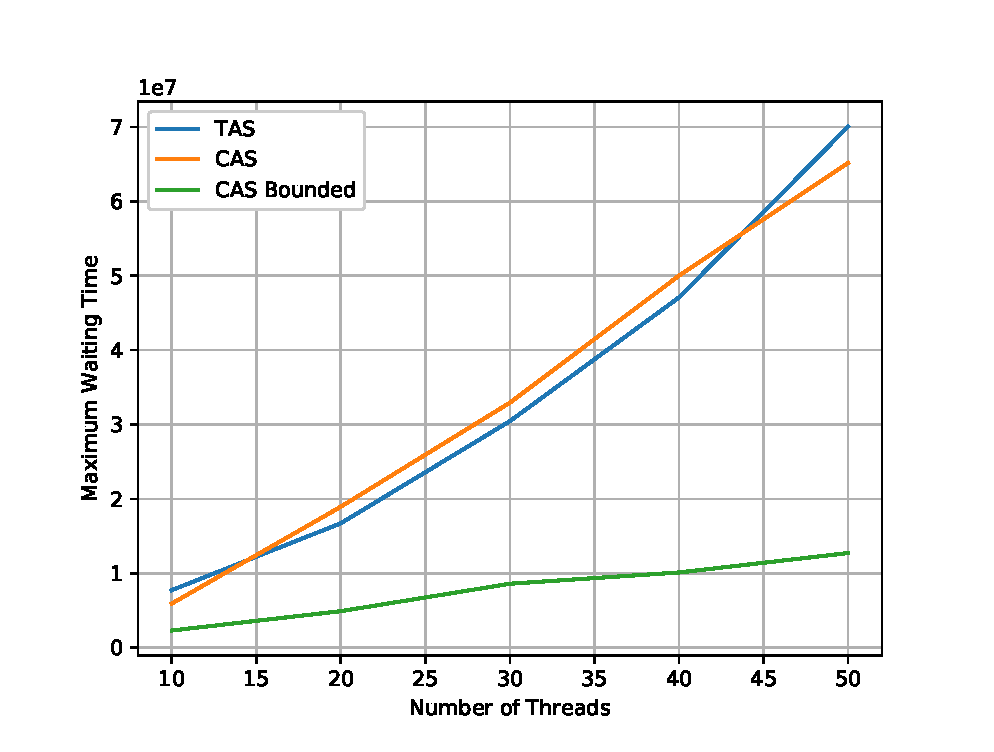
\includegraphics{max.eps}
\end{center}
\newpage
\section{Explaination of Results}
\end{document}